% 09_vacancies.tex -- Part 9, oxygen vacancies near W (register H-L). Sources: research_monograph/chapters/
% M10_w_and_vacancies.tex (sec:mono-w-hl, tab:mono-w-hl, fig:mono-w-hl, sec:mono-w-cells), M06_defect_theory.tex
% (sec:mono-defect-formation, eq:mono-defect-ef), M03_literature_materials.tex (sec:mono-lit-defects, sec:mono-lit-w);
% evidence/FACT_REGISTRY.tsv (FACT-050, FACT-051, FACT-052); research_record/03_CLAIMS_LEDGER.yaml (C038);
% qe_workflow/cern_htcondor/results/RESULTS_LOG.md (2026-10-13 03:40Z H-L entry: per-cell k3->k4 and width shifts);
% qe_workflow/analysis_2026-10-13_full/out/f11_hl_vacancy.json (all differences and per-cell changes);
% out/f13_hl_raw.json (In31WO48 k4: band above VB filled to 1.78 eV; monograph M06/M10 text rounds to 1.7 eV,
% FACT-043 gives 1.2-1.8 eV, so the slides write 1.7--1.8 eV).
% Figure: tools/fig_09_hl.py -> figures/09_hl_scores.pdf (data: out/f11_hl_vacancy.json, as monograph fig11_hl_vacancy).
% Binding wording: H-L is UNRESOLVED overall (never "supported"); dE_local(O30) significance unresolved; dE_dop passes
% under the registered settings only; spin sensitivity A20(i) staged, not run.
% Note: frame bodies start with a command, never with a brace group (beamer would read a subtitle).
\providecommand{\nineDloc}{\Delta E_{\mathrm{local}}}
\providecommand{\nineDdop}{\Delta E_{\mathrm{dop}}}
\providecommand{\nineVO}{V$_{\mathrm{O}}$}
% denser slides: footnotesize bullets, local to the frame in which it is called
\providecommand{\ninedense}{\setbeamerfont{itemize/enumerate body}{size=\footnotesize}%
  \setbeamerfont{itemize/enumerate subbody}{size=\footnotesize}}
% evidence label inside a \src line: same size as the surrounding \tiny text
\providecommand{\ninesrclab}[1]{[\textsc{\MakeLowercase{#1}}]}

\partslide{Part 9}{Oxygen vacancies near W}

% ---------------------------------------------------------------------------------------------------------------------
\begin{frame}{Test H-L was registered before any vacancy cell was built}
  \ninedense
  \begin{columns}[T,onlytextwidth]
    \begin{column}{0.47\textwidth}
      \centering
      \begin{tikzpicture}[x=1mm,y=1mm,font=\scriptsize,
          cellbox/.style={draw,line width=0.45pt,inner sep=1.0mm,align=center,minimum height=6.2mm},
          ref/.style={cellbox,text width=14mm},
          vac/.style={cellbox,text width=22mm},
          rm/.style={-{Stealth[length=1.6mm]},line width=0.5pt}]
        \node[ref] (h)  at (8,23)  {In$_{32}$O$_{48}$};
        \node[vac] (v)  at (42,23) {In$_{32}$O$_{47}$};
        \node[ref] (w)  at (8,7.5) {In$_{31}$WO$_{48}$};
        \node[vac] (fa) at (42,15) {In$_{31}$WO$_{47}$ \emph{far}};
        \node[vac] (ne) at (42,7.5)  {In$_{31}$WO$_{47}$ \emph{near}};
        \node[vac,dashed] (n7) at (42,0) {In$_{31}$WO$_{47}$ \emph{near72}};
        \draw[rm] (h) -- node[above,inner sep=0.7mm]{$-$O} (v);
        % one O removed from the W reference at three sites: a short bus, then one arrow per site
        \coordinate (bus) at ($(w.east)+(3.2,0)$);
        \draw[line width=0.5pt] (w.east) -- (bus);
        \draw[line width=0.5pt] (bus |- fa.west) -- (bus |- ne.west);
        \draw[line width=0.5pt,dashed] (bus |- ne.west) -- (bus |- n7.west);
        \draw[rm] (bus |- fa.west) -- node[above,inner sep=0.5mm]{$-$O32} (fa.west);
        \draw[rm] (bus |- ne.west) -- node[above,inner sep=0.5mm]{$-$O30} (ne.west);
        \draw[rm,dashed] (bus |- n7.west) -- node[above,inner sep=0.5mm]{$-$O72} (n7.west);
        \draw[{Stealth[length=1.4mm]}-{Stealth[length=1.4mm]},ntumaroon,line width=0.6pt]
          ($(fa.east)+(1.4,0)$) -- node[right,inner sep=0.7mm,text=ntumaroon]{$\nineDloc$} ($(ne.east)+(1.4,0)$);
      \end{tikzpicture}\par
      \vspace{0.6mm}
      {\footnotesize $\begin{aligned}
        \nineDloc &= E[\text{near}] - E[\text{far}]\\[-0.3mm]
        \nineDdop &= \big(E[\text{far}] - E[\mathrm{In_{31}WO_{48}}]\big)\\[-0.3mm]
          &\quad - \big(E[\mathrm{In_{32}O_{47}}] - E[\mathrm{In_{32}O_{48}}]\big)
      \end{aligned}$\par}
      \vspace{0.6mm}
      \raggedright{\scriptsize $E$: total energy of the neutral cell (left: 80 atoms, right: 79). Near and far share
        one composition and each bracket removes one O atom, so the O chemical potential cancels.\par}
      \src{This work, PAW-PBE (QE 7.3.1), 71/568\,Ry, Gaussian 0.005\,Ry, spin-unpolarised, fixed cell; relaxed on $3{\times}3{\times}3$
        ($k3$) to $10^{-3}$\,Ry/bohr, single points on $4{\times}4{\times}4$ ($k4$).}
    \end{column}
    \begin{column}{0.50\textwidth}
      \begin{itemize}
        \item Does W raise the energy of a neutral O vacancy, as the paper's statement that W passivates O
          vacancies would imply\sref[p.~4]{Januar2026}? Registered as amendment A17 (2026-10-10, 18:48Z), before any vacancy cell
          was built.
        \item Thresholds: $\nineDloc \ge +0.3$\,eV, $\nineDdop > +0.05$\,eV. Forecasts, not scored: $+0.5$ to
          $+1.5$\,eV and $+0.5$ to $+3$\,eV.
        \item Rules (A20): a $k3\to k4$ change $>10$\,meV means \emph{unresolved significance}; a spin or width
          (0.002\,Ry) sensitivity $>50$\,meV, or a flipped verdict, means \emph{not robust}.
        \item Sites: near = O30, the shortest W--O bond; O72, 0.01\,\AA{} longer, as a sensitivity (A19); far = O32,
          6.85\,\AA{} from W.
      \end{itemize}
    \end{column}
  \end{columns}
\end{frame}

% ---------------------------------------------------------------------------------------------------------------------
\begin{frame}{Both differences exceed their thresholds, yet H-L is unresolved}
  \ninedense
  \begingroup\scriptsize
  \setlength{\tabcolsep}{4.2pt}
  \renewcommand{\arraystretch}{1.1}
  \begin{tabularx}{\textwidth}{@{}l c c r r r r >{\raggedright\arraybackslash}X@{}}
    \toprule
    Difference & Rule & Forecast & $k3$, G 0.005 & $k4$, G 0.005 & $k3$, G 0.002 & $k3\to k4$ & Status (A20) \\
     & (eV) & (eV) & (eV) & (eV) & (eV) & (meV) & \\
    \midrule
    $\nineDloc$, O30 & $\ge +0.3$ & $+0.5$ to $+1.5$ & $+0.5578$ & $+0.5321$ & $+0.5583$ & $-25.7$ &
      significance \textsc{unresolved} \\
    $\nineDloc$, O72 & none & -- & $+0.6643$ & $+0.6230$ & $+0.6650$ & $-41.3$ & sensitivity, reported only \\
    $\nineDdop$ & $> +0.05$ & $+0.5$ to $+3$ & $+0.7259$ & $+0.7226$ & $+0.7261$ & $-3.4$ & \textsc{pass} (registered
      settings) \\
    \midrule
    \multicolumn{8}{@{}l}{Spin sensitivity A20(i): staged, not run (\textsc{unassessed}). \quad Overall: H-L
      \textbf{\textsc{unresolved}}.} \\
    \bottomrule
  \end{tabularx}\par\endgroup
  \src{This work, PAW-PBE (QE 7.3.1) \ninesrclab{computed}; O30: registered near site; G: Gaussian smearing width (Ry).
    An independent re-parse of the raw outputs gives the same energies.}
  \vspace{0.2mm}
  \begin{itemize}
    \item $\nineDloc$: a vacancy next to W costs a further 0.53--0.56\,eV, but the $k3\to k4$ change of
      $-25.7$\,meV breaks the 10\,meV rule: not a pass \lab{unresolved}.
    \item $\nineDdop$: in this degenerate crystalline cell W raises the energy of a neutral O vacancy far from it by
      0.73\,eV \lab{computed}.
    \item Width 0.002\,Ry shifts $\nineDloc$(O30) by $+0.5$\,meV and $\nineDdop$ by $+0.2$\,meV (rule: 50\,meV); spin was
      not run, so robustness is not established. Both outcomes lie inside the forecasts.
  \end{itemize}
  \takeaway{H-L is \textsc{unresolved}: $\nineDdop$ passes, $\nineDloc$ breaks the $k$-mesh rule, spin was not run.}
\end{frame}

% ---------------------------------------------------------------------------------------------------------------------
\begin{frame}{Per-cell $k$-mesh changes cancel in $\Delta E_{\mathrm{dop}}$ but not in $\Delta E_{\mathrm{local}}$}
  \ninedense
  \begin{columns}[T,onlytextwidth]
    \begin{column}{0.56\textwidth}
      \centering
      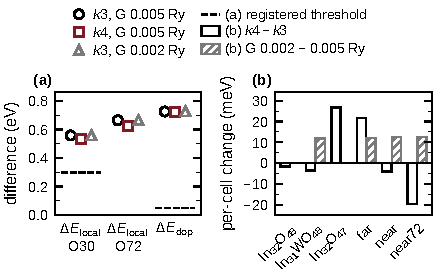
\includegraphics[width=0.97\linewidth]{09_hl_scores}\par
      \raggedright
      \src{(a) Differences on the three settings; dashed: registered thresholds (none for O72). (b) Per-cell change,
        $k4-k3$ (open) and G $0.002-0.005$\,Ry at $k3$ (hatched; 0.0 for the two W-free cells, so no bar). This work,
        PAW-PBE \ninesrclab{computed}; data: f11\_hl\_vacancy.json.}
    \end{column}
    \begin{column}{0.41\textwidth}
      \begin{itemize}
        \item $k3\to k4$ per cell: In$_{32}$O$_{47}$ $+26.8$, far $+21.6$, near $-4.1$, near72 $-19.7$\,meV;
          references In$_{32}$O$_{48}$ $-1.7$, In$_{31}$WO$_{48}$ $-3.5$\,meV \lab{computed}.
        \item $\nineDloc$ = near $-$ far: $-4.1 - 21.6 = -25.7$\,meV. In $\nineDdop$ the changes cancel to
          $-3.4$\,meV, which alone does not show that the energies are converged.
        \item Width 0.002\,Ry: each W cell $+11.7$ to $+12.6$\,meV, the pure cells 0.0\,meV; this cancels in the
          differences.
        \item All six relaxations converged; the near cell needed one restart under the pre-declared rule A28.
      \end{itemize}
    \end{column}
  \end{columns}
  \takeaway{The $k$-mesh rule, not the threshold, leaves $\Delta E_{\mathrm{local}}$ unresolved.}
\end{frame}

% ---------------------------------------------------------------------------------------------------------------------
\begin{frame}{Neither difference is a formation energy at a device Fermi level}
  \ninedense\toggletrue{blx@useprefix}% print "Van de Walle" in the footnote (local to this frame)
  {\small\centering $\displaystyle E^{f}[X^{q}](\EF) = E_{\mathrm{tot}}[X^{q}] - E_{\mathrm{tot}}[\mathrm{host}]
    - \sum\nolimits_i n_i\mu_i + q\,(\EF + E_{\mathrm{VBM}}) + E_{\mathrm{corr}}[X^{q}]$%
    \srefs{VandeWalle2004,Freysoldt2014}\par}
  {\scriptsize\raggedright where $E_{\mathrm{tot}}$: total energy of the cell with defect $X$ (charge $q$) or of the host;
    $n_i$ atoms of chemical potential $\mu_i$ added ($n_i>0$) or removed; $\EF$ measured from the valence-band maximum
    $E_{\mathrm{VBM}}$; $E_{\mathrm{corr}}$: image-charge and potential-alignment correction.\par}
  \vspace{0.3mm}
  \begin{columns}[T,onlytextwidth]
    \begin{column}{0.34\textwidth}
      \centering
      \begin{tikzpicture}[x=1mm,y=1mm,font=\scriptsize]
        % (left) W cell as computed: host band filled to 1.7-1.8 eV above its bottom (schematic; 8 mm per eV)
        \fill[rulegrey!60] plot[domain=-4.76:4.76,samples=40] (\x,{0.6*\x*\x}) -- cycle;
        \draw[line width=0.6pt] plot[domain=-5.8:5.8,samples=50] (\x,{0.6*\x*\x});
        \draw[line width=0.4pt] (-7.5,0) -- (7.5,0) node[right,inner sep=0.5mm]{$\Ec$};
        \draw[dashed,line width=0.5pt] (-7.5,13.6) -- (7.5,13.6) node[right,inner sep=0.5mm]{$\EF$};
        \draw[{Stealth[length=1.2mm]}-{Stealth[length=1.2mm]},line width=0.4pt] (-6.6,0.4) --
          node[left,inner sep=0.5mm,align=right]{1.7--\\1.8\,eV} (-6.6,13.2);
        \draw[-{Stealth[length=1.4mm]},ntumaroon,line width=0.6pt] (4.2,20.2) -- (2.0,14.2);
        \node[anchor=south west,text=ntumaroon,inner sep=0.3mm] at (2.3,20.2) {\nineVO{} electrons};
        \node[anchor=north] at (0,-1.2) {W cell (computed)};
        % (right) device film: E_F below the band edge (inferred, not computed)
        \begin{scope}[xshift=23mm]
          \draw[line width=0.6pt] plot[domain=-5.8:5.8,samples=50] (\x,{0.6*\x*\x});
          \draw[line width=0.4pt] (-6,0) -- (6,0) node[right,inner sep=0.5mm]{$\Ec$};
          \draw[dashed,line width=0.5pt] (-6,-3.6) -- (6,-3.6) node[right,inner sep=0.5mm]{$\EF$};
          \node[anchor=north] at (0,-4.6) {device film};
        \end{scope}
      \end{tikzpicture}\par
      \raggedright
      \src{Schematic; only the 1.7--1.8\,eV filling of the W cell is computed. At device densities $\EF$ lies below
        $\Ec$ \ninesrclab{inferred}.}
    \end{column}
    \begin{column}{0.63\textwidth}
      \begin{itemize}
        \item Band filling: the vacancy electrons enter a band already filled to 1.7--1.8\,eV, so $\nineDdop$ mixes
          filling with chemistry, strain and image terms. At device densities this term would be much smaller
          \lab{inferred}; its sign and size there are not computed.
        \item Cell-limited: the far site is only 6--8\,\AA{} from W and its images, so $\nineDloc$ is a cell-limited
          estimate.
        \item No charged state, $E_{\mathrm{corr}}$ or hybrid functional: no charge-transition level; how deep
          \nineVO{} lies is debated\srefs{Agoston2009,Buckeridge2018,Chatratin2019}.
        \item Crystalline cells; the films are amorphous or nanocrystalline. $\nineDdop$ has the sign that vacancy
          passivation by W\sref[p.~4]{Januar2026} implies, but neither supports nor tests it for the films.
      \end{itemize}
    \end{column}
  \end{columns}
  \takeaway{H-L is a crystalline reference at degenerate filling, not a test of the device films.}
\end{frame}
